\documentclass[10pt]{beamer}
\usepackage[utf8]{inputenc}
\usepackage{xeCJK}
\usepackage{graphicx}
\usepackage{mathtools}
\usepackage{utopia} %font utopia imported
\usetheme{CambridgeUS}
\usecolortheme{dolphin}

\setCJKmainfont[AutoFakeBold,ItalicFont=KaiTi]{SimHei}%
\setCJKsansfont[AutoFakeBold]{SimHei}%
\setCJKmonofont{FangSong}

% set colors
\definecolor{myNewColorA}{RGB}{176,32,60}
\definecolor{myNewColorB}{RGB}{215,105,104}
\definecolor{myNewColorC}{RGB}{253,178,147}
\setbeamercolor*{palette primary}{bg=myNewColorC}
\setbeamercolor*{palette secondary}{bg=myNewColorB, fg = white}
\setbeamercolor*{palette tertiary}{bg=myNewColorA, fg = white}
\setbeamercolor*{titlelike}{fg=myNewColorA}
\setbeamercolor*{title}{bg=myNewColorA, fg = white}
\setbeamercolor*{item}{fg=myNewColorA}
\setbeamercolor*{caption name}{fg=myNewColorA}
\usefonttheme{professionalfonts}
\usepackage{natbib}
\usepackage{hyperref}
%------------------------------------------------------------
\titlegraphic{
\includegraphics[height=1.5cm]{xdu.png}}

\setbeamerfont{title}{size=\large}
\setbeamerfont{subtitle}{size=\small}
\setbeamerfont{author}{size=\small}
\setbeamerfont{date}{size=\small}
\setbeamerfont{institute}{size=\small}

\AtBeginSection[]{
  \begin{frame}
  \vfill
  \centering
  \begin{beamercolorbox}[sep=8pt,center,shadow=true,rounded=true]{title}
    \usebeamerfont{title}\insertsectionhead\par%
  \end{beamercolorbox}
  \vfill
  \end{frame}
}

\begin{document}

\title{基于同态加密的用户交易金额隐私保护方案}
\subtitle{毕业设计 答辩展示}
\author[黄**]{
  \begin{tabular}{rl}
    答辩学生:& 黄** \\
    指导老师:& 王**
  \end{tabular}
}
\institute[camber@poi.science]{西安电子科技大学}
\date[2023.5.29]{2023.5.29}

% Table of contents
\frame{\titlepage}
\begin{frame}{目录}
    \tableofcontents
\end{frame}

% 01-intro.tex
% about 2-3mins
\section{课题综述}

\subsection{选题背景和研究意义}

\begin{frame}
    \frametitle{选题背景}

    % 背景包括
    \begin{itemize}
        \item 移动支付随着电子商务的兴起而被推广:
        \begin{itemize}
            \item 买卖双方在线下商定好金额后,通过某一支付服务提供商进行转账;
            \item 依托于云计算服务
        \end{itemize}
        \item 受到许多安全方面的挑战:
        \begin{itemize}
            \item 外部:攻击者通过各种方式获得密钥并解密信息,或是“先存储后解密”攻击;
            \item 内部:监守自盗,在未经用户许可下访问信息并非法构建用户画像;
        \end{itemize}
        \item 泄露后果:推断用户其他各种敏感信息
    \end{itemize}

\end{frame}

\begin{frame}
    \frametitle{研究意义}

    本文提出了一种金额密态的,适用于移动支付场景的交易方案,实现了用户之间的交易金额只由交易双方知道而不泄露给第三方。具体而言:
    \begin{itemize}
        \item 借助 CKKS 方案所基于的困难问题,保证交易金额的隐私性;
        \item 使用 CKKS 方案的同态特性,实现了对用户密文账户余额的同态操作以及手续费的计算,确保了可交易性;
        \item 本文的研究有助于拓展和提出更完备、功能更强的交易隐私保护方案,也有助于提高用户对移动支付的信任度。
    \end{itemize}

\end{frame}

\subsection{研究现状}

\begin{frame}
    \frametitle{相关工作}

    \begin{itemize}
        \item 全同态加密
        \begin{itemize}
            \item Craig G. 首次提出整数的全同态加密方案,包括自举手段等
            \item Cheon 等人在 2017 年提出支持浮点数加解密的同态加密方案 HEAAN,并被后人学者命名为 CKKS,通过自举达到全同态性。
        \end{itemize}
        \item 隐私交易方案 
        \begin{itemize}
            \item 2018 年,一个结合了区块链和同态加密的电子医疗记录隐私保护方案被提出,实现了保险公司等第三方在无法获取客户明文医疗记录的情况下,仍然可以判断是否理赔的功能;
            \item 2020 年,姜轶涵等人在他的文献里运用了同态加密、零知识证明和数字签名等密码学手段,提出了一个密态的可审计交易方案。
        \end{itemize}
    \end{itemize}

\end{frame}

\subsection{主要贡献和创新}

\begin{frame}
    \frametitle{主要贡献和创新}

    \begin{itemize}
        \item 对现有的交易隐私保护方法和全同态加密算法进行调研,提出了一个基于同态加密的用户交易金额隐私保护交易方案;
        \item 使用 CKKS 方案对浮点数的支持的特性,确保了交易的隐私性和可交易性,包括浮点数手续费的计算,以及账户密文余额同态更新等;
        \item 使用密钥交换确保了交易的正确性;使用 ECDSA 算法确保了不可伪造性;
        \item 使用 Golang 编写了一个简单的库实现,包括客户端和服务端逻辑、一个简单的服务器 CLI 程序,以及相关单元测试;
        \item 测试表明,方案在密码学方面具有良好的时间开销和可以接受的空间开销。
    \end{itemize}

\end{frame}

\subsection{论文结构安排}
\begin{frame}
    \frametitle{论文结构安排}

    \begin{enumerate}
        \item 绪论
        \item 基础知识
        \item 支付方案设计
        \item 具体的代码设计
        \item 实验评估
        \item 总结和展望
    \end{enumerate}

\end{frame}


\section{方案设计}

\subsection{技术路线}

\begin{frame}
    \frametitle{技术路线}

    \begin{itemize}
        \item 编程语言:Golang
        \item 密码学库:crypto/ecdsa, \texttt{github.com/tuneinsight/lattigo/v4}
        \item 数据库:SQLite3,及 \texttt{github.com/mattn/go-sqlite3}
    \end{itemize}

\end{frame}

\begin{frame}
    \frametitle{数据库设计}

    \begin{figure}[h]
        \centering
        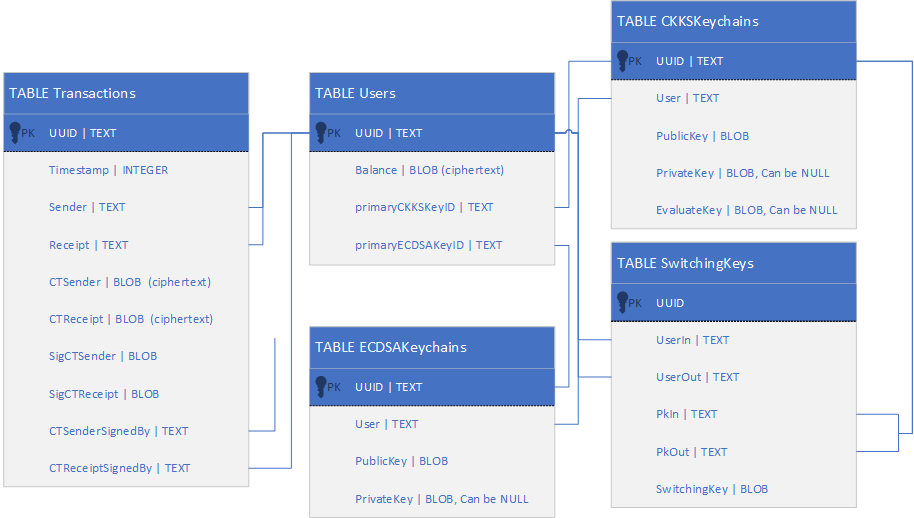
\includegraphics[width=0.8\linewidth]{figures/chimata-database-design.png}
        \caption{数据库设计抽象}
    \end{figure}

\end{frame}

\subsection{交易流程描述}

\begin{frame}
    \frametitle{交易流程 - 总体}

    \begin{figure}[h]
        \centering
        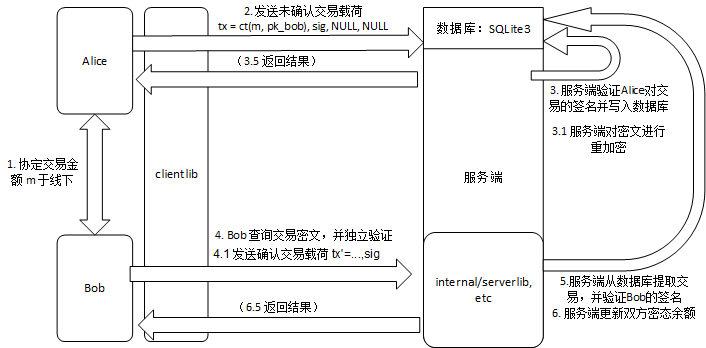
\includegraphics[width=0.75\linewidth]{figures/Tx-Abstract.png}
    \end{figure}

    此外方案代码也提供了一个以转出方公钥加密的交易发起的实现,和下文类似,仅无确认流程。这里不再赘述。
\end{frame}

\begin{frame}
    \frametitle{交易流程 - 转出方发起}

    \begin{itemize}
        \item Alice 与 Bob 协定交易金额 $m$
        \item Alice 通过以下调用方法,向服务端发送请求:
        \begin{itemize}
            \item 以用户 bob 和交易金额 $m$ 为参数调用 \texttt{alice.TransferByReceiptPK(bob, m)} 以生成需要提交的交易结构体 \newline 包括加密交易金额和对密文签名,生成交易载荷 $tx = \{NULL, NULL, ct_b, sig\}$
            \item 调用 \texttt{alice.CreateTransferJob(tx)} 和服务端进行网络交互 \newline 将交易载荷反序列化为 JSON,通过 http 发送到服务端接口 \texttt{(server)/transaction/create/byReceiptPK}
            
        \end{itemize}
    \end{itemize}

\end{frame}

\begin{frame}
    \frametitle{交易流程 - 服务端验证和重加密}

    \begin{itemize}
        \item 服务端接收到交易发起请求,调用方法 \texttt{HandlerTransactionCreateByReceiptPK}
        \begin{itemize}
            \item 使用 Alice 的 ECDSA 公钥对交易密文的签名进行验证
            \item 使用 $swk_{Bob \rightarrow Alice}$ 进行重加密
            \item 写入数据库,向 Alice 返回结果,包括分配的 uuid 等 
        \end{itemize}
        \item 若服务端任何一处出现问题,则返回非 200 代码,包含具体错误于键值对 \texttt{"error": (actual error message)} 中。
    \end{itemize}

\end{frame}

\begin{frame}
    \frametitle{交易流程 - 转入方确认和服务端更新账户}

    \begin{itemize}
        \item Bob 可以以 uuid 向服务端查询交易,获得交易信息 \texttt{txNew},并验证是否金额是否正确
        \item Bob 对交易中以 Alice 的公钥加密的密文进行签名,并提交给服务器
        \begin{itemize}
            \item 调用 \texttt{bob.AcceptTransactionByTransaction(txNew)} 进行签名的生成
            \item 调用 \texttt{bob.CreateConfirmTransactionTask(txNew)} 将签名后的交易发送给服务端接口 \texttt{(server)/transaction/confirm},等待回应
        \end{itemize}
        \item 服务端接收到交易接受请求,进行验证;
        \item 服务端更新交易双方密文余额,并写入数据库
        \begin{itemize}
            \item 即:对转出方密态余额减去交易金额,对转入方密态余额加上交易金额。
        \end{itemize}
    \end{itemize}

\end{frame}

\subsection{方案相关分析}

\begin{frame}
    \frametitle{分析}

    \begin{itemize}
        \item 隐私性:由 CKKS 方案保证
        \begin{itemize}
            \item R-LWE 问题:归约至 SVP 问题,NP-Hard,and post-quantum
        \end{itemize}
        \item 不可伪造性:由 ECDSA 签名方案保证:
        \begin{itemize}
            \item 交易双方对密文摘要进行签名
            \item 伪造是困难的
        \end{itemize}
        \item 可交易性与正确性:由基于 R-LWE 假设的加密方案的相关性质保证
        \begin{itemize}
            \item 浮点数的同态性:保证了可以正确更新密态余额和计算手续费
            \item R-LWE 的密钥交换方法:正确性
        \end{itemize}
    \end{itemize}

\end{frame}

\section{实验结果与分析}

\subsection{实验过程与结果}

\begin{frame}
    \frametitle{实验环境}

    \begin{itemize}
        \item 操作系统:Arch Linux
        \item Golang 工具链:版本 1.20.4,Arch 软件包仓库版本 \texttt{go 2:1.20.4-1};
        \item 处理器:AMD Ryzen 9 4900HS (16) @ 3.000GHz,插入电源;
        \item 内存:16 GB,以及 32 GB 的 Linux 交换空间; 
        \item 安全参数:
        \begin{itemize}
            \item CKKS: PQ12QP109
            \item ECDSA: NIST P-224
        \end{itemize}
    \end{itemize}

\end{frame}

\begin{frame}
    \frametitle{测试描述}

    \begin{itemize}
        \item 客户端:通过 Golang 工具链自带的测试框架,进行相应函数和功能的集成测试和性能评估;\newline 测试内容包括了生成交易的正确性和时间开销、和服务端交互的时间开销等
        \begin{itemize}
            \item 以默认参数执行测试:\texttt{go test -v ./internal/{clientlib,serverlib}}
            \item 以默认参数执行性能测试:\texttt{go test -bench . ./internal/{clientlib,serverlib}}
        \end{itemize}
        \item 服务端:对服务端的测试大部分被包括在了客户端测试中的服务端交互部分,少部分函数单独写了测试和 Benchmark;
    \end{itemize}

\end{frame}

\begin{frame}
    \frametitle{实验结果记录 - Benchmark 截图}

    \begin{figure}
        \centering
        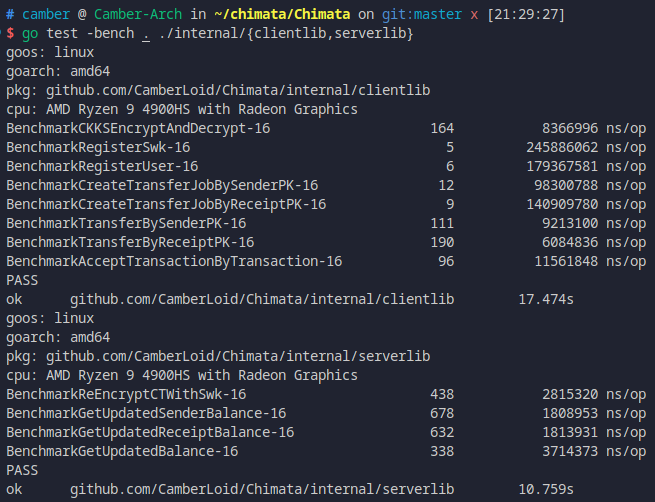
\includegraphics[width=0.8\linewidth]{figures/Bench_Overall.png}
        \caption{Benchmark 截图}
    \end{figure}

\end{frame}

\subsection{实验结果分析}
 
\begin{frame}
    \frametitle{时间开销分析}

    对时间开销的实验数据收集后,汇总如下图:

    \begin{table}[h]
        \begin{tabular}{|l|c|c|c|c|}
            \hline
            类别 & 单笔交易 & 加解密与重加密 & 密态余额更新 & 数据库操作 \\
            \hline
            平均消耗时间 & 105 ms & 15 ms & 4.5 ms & 75.5 ms \\ 
            \hline
            百分比 & 100.0\% & 14.2\% & 4.3\% & 71.9\% \\
            \hline
        \end{tabular}
        \caption{各部分时间开销与单笔交易开销的关系}
    \end{table}

    \begin{itemize}
        \item CKKS 方案相关函数:在指定的安全参数下表现优秀,约 20ms 每笔交易;
        \item 数据库:主要时间开销,有较大优化空间。
        \item 其他:网络交互处理、签名验证等
    \end{itemize}

    %综合上述测试结果,服务端对单笔交易两个不同的方法的平均处理和返回时间约为 105 ms,其中 CKKS 方案的密码学相关函数占比约为 20\%,可以认为在选择的安全参数下,本文的同态加密核心部分工作性能良好。而 CKKS 方案的密码学函数以外的时间开销以数据库操作为主,占据了单笔交易的大部分处理时间,约为 70\%,未来的优化方向可以从这方面入手。其他开销约占比 10\%,包括了网络交互开销和签名验证开销等。

\end{frame}

\begin{frame}
    \frametitle{空间开销分析}

    服务端在处理交易信息后,其存储的密文的数据库大小,即服务端的空间开销进行评估。对实验结果进行收集后绘制如下图:

    \begin{figure}[h]
        \centering
        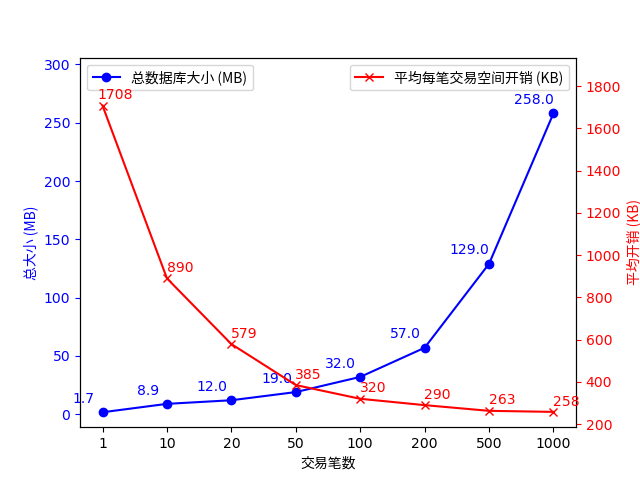
\includegraphics[width=0.8\linewidth]{./figures/Bench_DatabaseSize.png}
        \caption{交易方案的空间开销测试数据}
    \end{figure}

\end{frame}


\begin{frame}
    \frametitle{空间开销分析 - Cont}

    \begin{itemize}
        \item 当交易笔数为 1000 时的约 258 KB 每笔交易,推算,每 1 GB 空间可以存储约 4000 笔交易信息;
        \item 考虑到目前计算机存储成本越来越低,可以认为本文所提出的服务端实现具有较高的空间效率,具有可实现性;
        \item 未引入数据压缩算法:可以预期较大的空间效率提升,如 gzip。
    \end{itemize}

\end{frame}

\section{总结与展望}

\begin{frame}
    \frametitle{研究总结}

    \begin{itemize}
        \item 对现有的交易隐私保护方法和全同态加密算法进行了简要的调研;
        \item 对全同态加密库 Lattigo 和 CKKS 方案的使用方法和相关特性进行研究;
        \item 对提出方案进行了简要的性能基准测试,证明了其可实现性;
        \item 展望:部署至真实云端
    \end{itemize}

\end{frame}

\section*{提问}


\end{document}
